\documentclass[../main.tex]{subfiles}
\graphicspath{{\subfix{../../images/}}}
\begin{document}


\chapter{Task Performance}\label{chap:performance}

\begin{quote}
    \emph{Because some tasks require that certain components be mastered before other components can be performed or even attempted, there is likely to be a typical developmental sequence in acquiring certain skills. Furthermore, if substantial work is required for component processes to reach a level of mastery before higher level tasks can be attempted, then there is likely to be some period of consolidation in the acquisition of the higher level skill. That is, there will be periods in which there appears to be little progress being made in performance of the task. Closer scrutiny, however, may reveal that performance is improving, but only on lower level components of the task. According to this view of skill acquisition, then, the processes that underlie plateaus in learning curves may also underlie the stages that are characteristic of cognitive development}\\
    \raggedleft{--- Jean Piaget, 1953}
\end{quote}


% \begin{quote}
%     \emph{Perception is not something that happens to us, or in us, \lbrack\ldots\rbrack It is something we do.}\\ 
%     \raggedleft{--- Alva Noë, Perception in Action}
% \end{quote}

% \begin{quote}
%     \emph{The motor learning field does not yet possess an adequate computational model for practice-induced increases in motor acuity.}\\
%     \raggedleft{--- Krakauer et al. 2019}
% \end{quote}

\cleardoublepage%


\section{Performance over Blocks}\label{sec:performance_over_blocks}

Since we have verified that the methods of our task are sounds, our next question is whether subjects are in fact learning to achieve the goals of the tasks. As our intention is to ``stretch'' learning across the task, we can generate learning curves to understand if we met this aim. As visualized in \Cref{fig:hits_and_noholds}, we find that subjects, based on numbers of target ``hits'' (reaching the target with the cursor in the allotted time constraint), are learning over trials to increase their performance. These results over subjects immediately pose further questions. As there is a variety across subjects in the speed of learning-- some subjects appear to achieve the goals of the task rapidly (see the best performing subject hitting nearly every target after just 8 blocks, or 96 trials) while others struggle to reach more than half the targets on average (see the worst performing subject) throughout their session. Most subjects, however (see the median subject), show a rise in performance across their session, indicating that the task does in fact ``stretch'' the learning process in time, providing an opportunity to observe the features of learning over trials. Few subjects are unable to ``hold'' in the task, and these issues were quickly addressed (often by a minor adjustment in the electrode assembly to remove an electrical artifact).

\begin{figure}[!htb]%[H]
    \centering
    \includegraphics[width=1.0\textwidth]{basic_results/performance_over_blocks/hits_and_noholds.pdf}
    \caption[Hit and No-Hold counts over trials]{Target task outcomes over 45 blocks of 12 unique targets each, in randomized order per block. Subjects with the most, median, and least number of hits out of all 46 subjects are shown in green, blue, and orange, respectively. All other subjects are show in gray. Top: the number of ``Hits'' (reaching the target within the allotted time window after holding in the center of the task screen) within each block. Bottom: the number of ``No-Holds'' (occurs when a subject is unable to initiate trial by keeping the cursor in the center of the task screen for the allotted time. High numbers of No-Holds resulted in minor adjustments to the recoding apparatus to rectify any issues).}\label{fig:hits_and_noholds}
\end{figure}

Hit count is not the only measure of performance. As a ``hit'' implies decreasing the distance in task space between the target and the cursor (referred to as ``task error''), we defined ``mean reward'' over $K$ trials and $T$ timepoints using the inverse of the 2-norm of the distance between the cursor position $x$ and the target position $g$ for a given timepoint $t$ and trial $k$:

\begin{align}
    r = \frac{1}{KT}\sum_k^K\sum_t^T{|| \vec{g_k} - \vec{x}_{t,k} ||^{-2}}.
    \label{eq:reward}
\end{align}

That is, as subjects deviate further, on average, from their targets, the are ``rewarded'' according to an inverse square of their ``error''. We refer to this henceforth as task ``error''. Note that this notion of reward is calculated using the ``active'' samples as defined in \Cref{chap:methods}. Histograms of reward and hit counts per subject are shown in \Cref{fig:reward_histograms}. Where the hit counts are skewed, the mean rewards over subjects are approximately normal. In \Cref{fig:hit_fraction_vs_reward}, we find evidence that supports a linear correlation between this notion of reward and number of hits, as we would expect ($p=\num{0.978e-9}$). Put simply, hits can happen with more or less reward, and reward is a more fine-grained signal of performance as it reflects the trajectory directly as opposed to the binary outcome of each movement. Higher reward implies more direct, straight-line trajectories to targets. The residuals here imply that subjects miss their targets by deviating further from their targets in all directions, as opposed to repeated, systematic errors. This is supported in the bottom plot of \Cref{fig:hit_fraction_vs_reward}, where we see evidence that the standard deviation of the task error decreases with higher-hit-count subjects. Subjects who hit more targets are less varied in their trajectories than those who achieve fewer hits, providing support for the idea that subjects suffer from general task variability rather than systematic error. We explore the nature of this variability more deeply in later sections.

\begin{figure}[!htb]%[H]
    \centering
    \begin{minipage}{0.49\textwidth}
        \includegraphics[width=0.9\textwidth]{basic_results/trial_reward/reward_histogram.pdf}
        \subcaption{}
    \end{minipage}
    \begin{minipage}{0.49\textwidth}
        \includegraphics[width=0.9\textwidth]{basic_results/trial_reward/hit_fraction_histogram.pdf}
      \subcaption{}
    \end{minipage}
    \caption[Hit and reward histograms]{(a) Histogram over subjects of mean rewards as described in the main text. (b) Histogram over subjects of the fraction of trials which are hit trials.}\label{fig:reward_histograms}
\end{figure}

\begin{figure}[!htb]%[H]
    \centering
    \includegraphics[width=1.0\textwidth]{basic_results/performance_over_blocks/hit_fraction_vs_reward.pdf}
    \caption[Hits versus reward]{Hit counts versus total reward. Reward is calculated as shown in \cref{eq:reward}.}\label{fig:hit_fraction_vs_reward}
\end{figure}

We hypothesized that subjects who achieved more hits in the task would reduce the time it took them to hit those targets across their trials. This is visualized in \Cref{fig:reach_times_over_blocks}, where we see qualitative evidence supporting this idea; the highest performing subject tends to decrease their hit times over trials, while lesser performing subjects tend to take longer to move on average in each block; the lowest performing subject does not tend to decrease their reach time. This evidence extends to two other task metrics: path length, shown in \Cref{fig:path_length_over_blocks}, and number of path segments, shown in \Cref{fig:path_segments_over_blocks}. Path length is computed as the sum of the euclidean distance between each timestep. 

Path segments, as demonstrated in \Cref{fig:example_segments}, are defined as points where the sign of the task trajectory's derivative changes, or ``zero crossings'' of the derivative. We filter low-velocity zero crossings and combine crossings that are close to one another to ensure segments reflect natural ``syllables'' of movement. We used this definition of trajectory segments to investigate the concept of degree-of-freedom freezing, initially suggested by Bernstein as a first phase of motor learning \cite{Bernstein1967}. We see qualitatively across all subjects a reduction in path segmentation, though it is not dramatic. We also see that on average higher performing subjects have fewer path segments than their lower performing counterparts, implying smoother, more fluid movements combining motor actions or syllables in concert over time to reach targets. As we will see in later sections, subjects tend to blend their modal activities into solutions for each target over learning. We can speculate that the 2D task projection of subject EMG activities may mask degree-of-freedom freezing. We suggest a further investigation of this idea in the EMG data directly, perhaps tracking orthogonal EMG subspaces over time within trials. EMG subspaces is a different, perhaps more illuminating, definition of degree of freedom. We will investigate EMG subspaces over trials in later sections.

While we find qualitative evidence that these metrics correlate as expected with reward, only path length versus reward ($p=\num{2.2e-2}$) and path segments versus reward ($p=\num{4.5e-2}$) reveal (slight) statistical significance, as shown in \Cref{fig:reward_v_metrics} when looking across all subjects. These comparisons are computed using the percent difference between the means of the first and last groups of 15 blocks (180 trials) for each metric. We hypothesize that reach time shows an insignificant correlation as the trial time window was long enough (5s), subjects were not time-pressured and thus did not overly factor movement time into their strategies. These results highlight the variability of each subject; each individual is likely to have a unique strategy or objective associated with the task, and these coarse metrics fail to immediately capture the nuances of each subjects' movement patterns across learning. This is taken as a positive sign, that the features of this data are rich, and not easily captured by statistics which average out subjects' individual learning trajectories.

\begin{figure}[!htb]%[H]
    \centering
    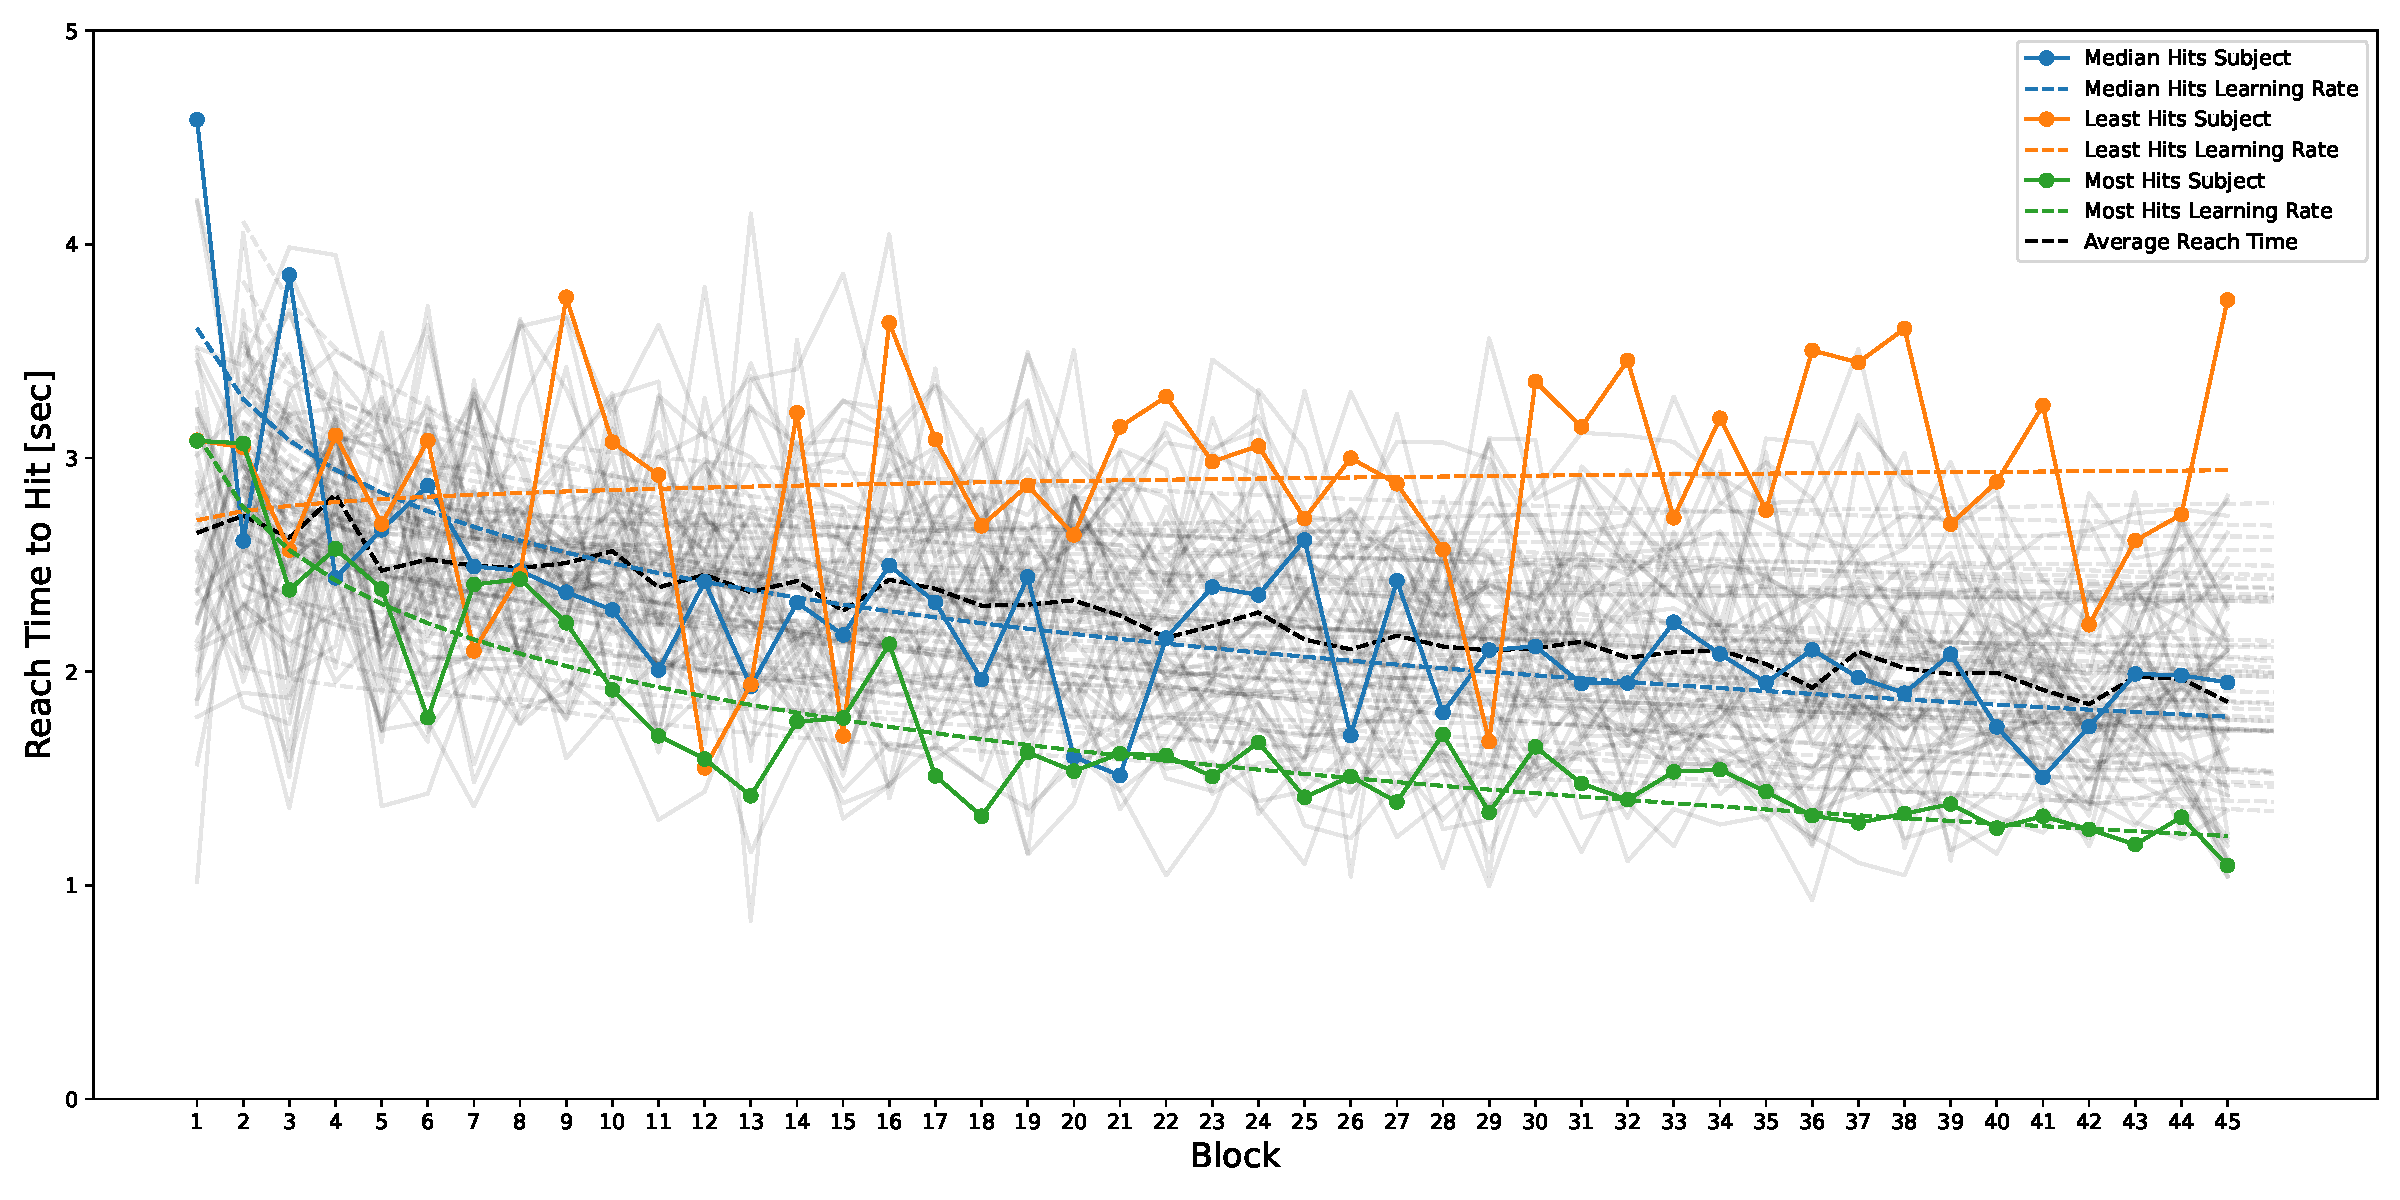
\includegraphics[width=1.0\textwidth]{basic_results/performance_over_blocks/reach_times_over_blocks.pdf}
    \caption[Reach time over blocks]{Reach time, measured using timers during the experimental sessions, averaged over each subjects' block of 12 trials, one trial per target in randomized order. Subjects with the most, least, and median numbers of hits are shown in green, orange, and blue, respectively. Log-fits are shown in matching colors for each of these subjects are shown to guide the eye. The mean over subjects per block is shown in dotted black.}\label{fig:reach_times_over_blocks}
\end{figure}

% return np.sum (np.sqrt (np.sum (np.diff (a, axis=0)**2,axis=1)))
\begin{figure}[!htb]%[H]
    \centering
    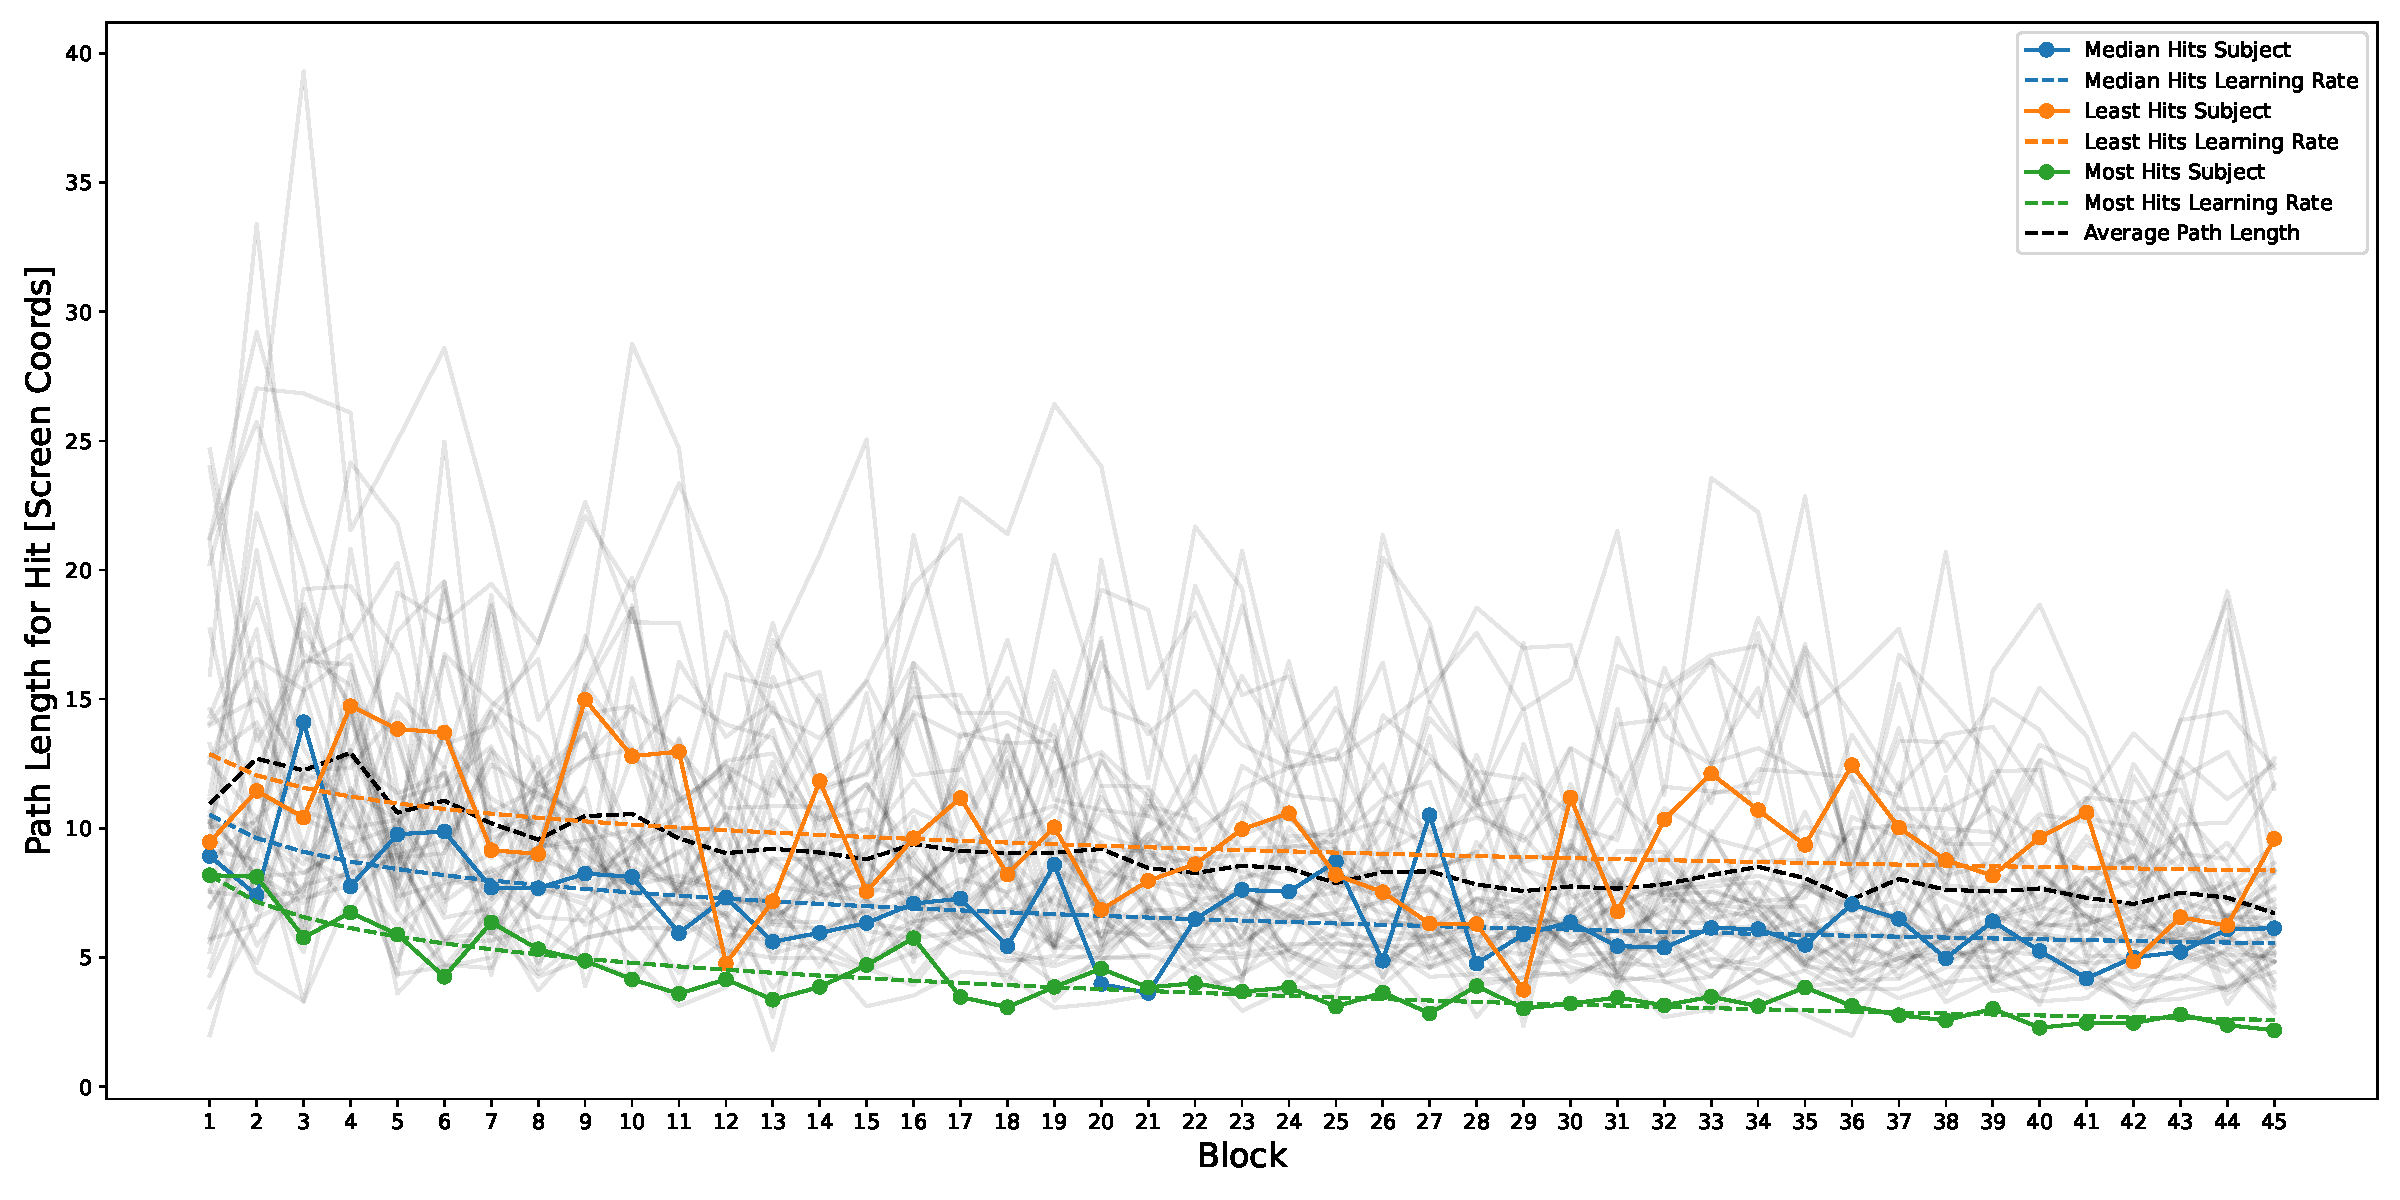
\includegraphics[width=1.0\textwidth]{basic_results/performance_over_blocks/path_length_over_blocks.pdf}
    \caption[Trajectory length over blocks]{Trajectory length in task space, computed as the sum of the squares of the trajectory finite difference over time, averaged over each subjects' block of 12 trials, one trial per target in randomized order. Subjects with the most, least, and median numbers of hits are shown in green, orange, and blue, respectively. Log-fits are shown in matching colors for each of these subjects are shown to guide the eye. The mean over subjects per block is shown in black dotted line.}\label{fig:path_length_over_blocks}
\end{figure}

\begin{figure}[!htb]%[H]
    \centering
    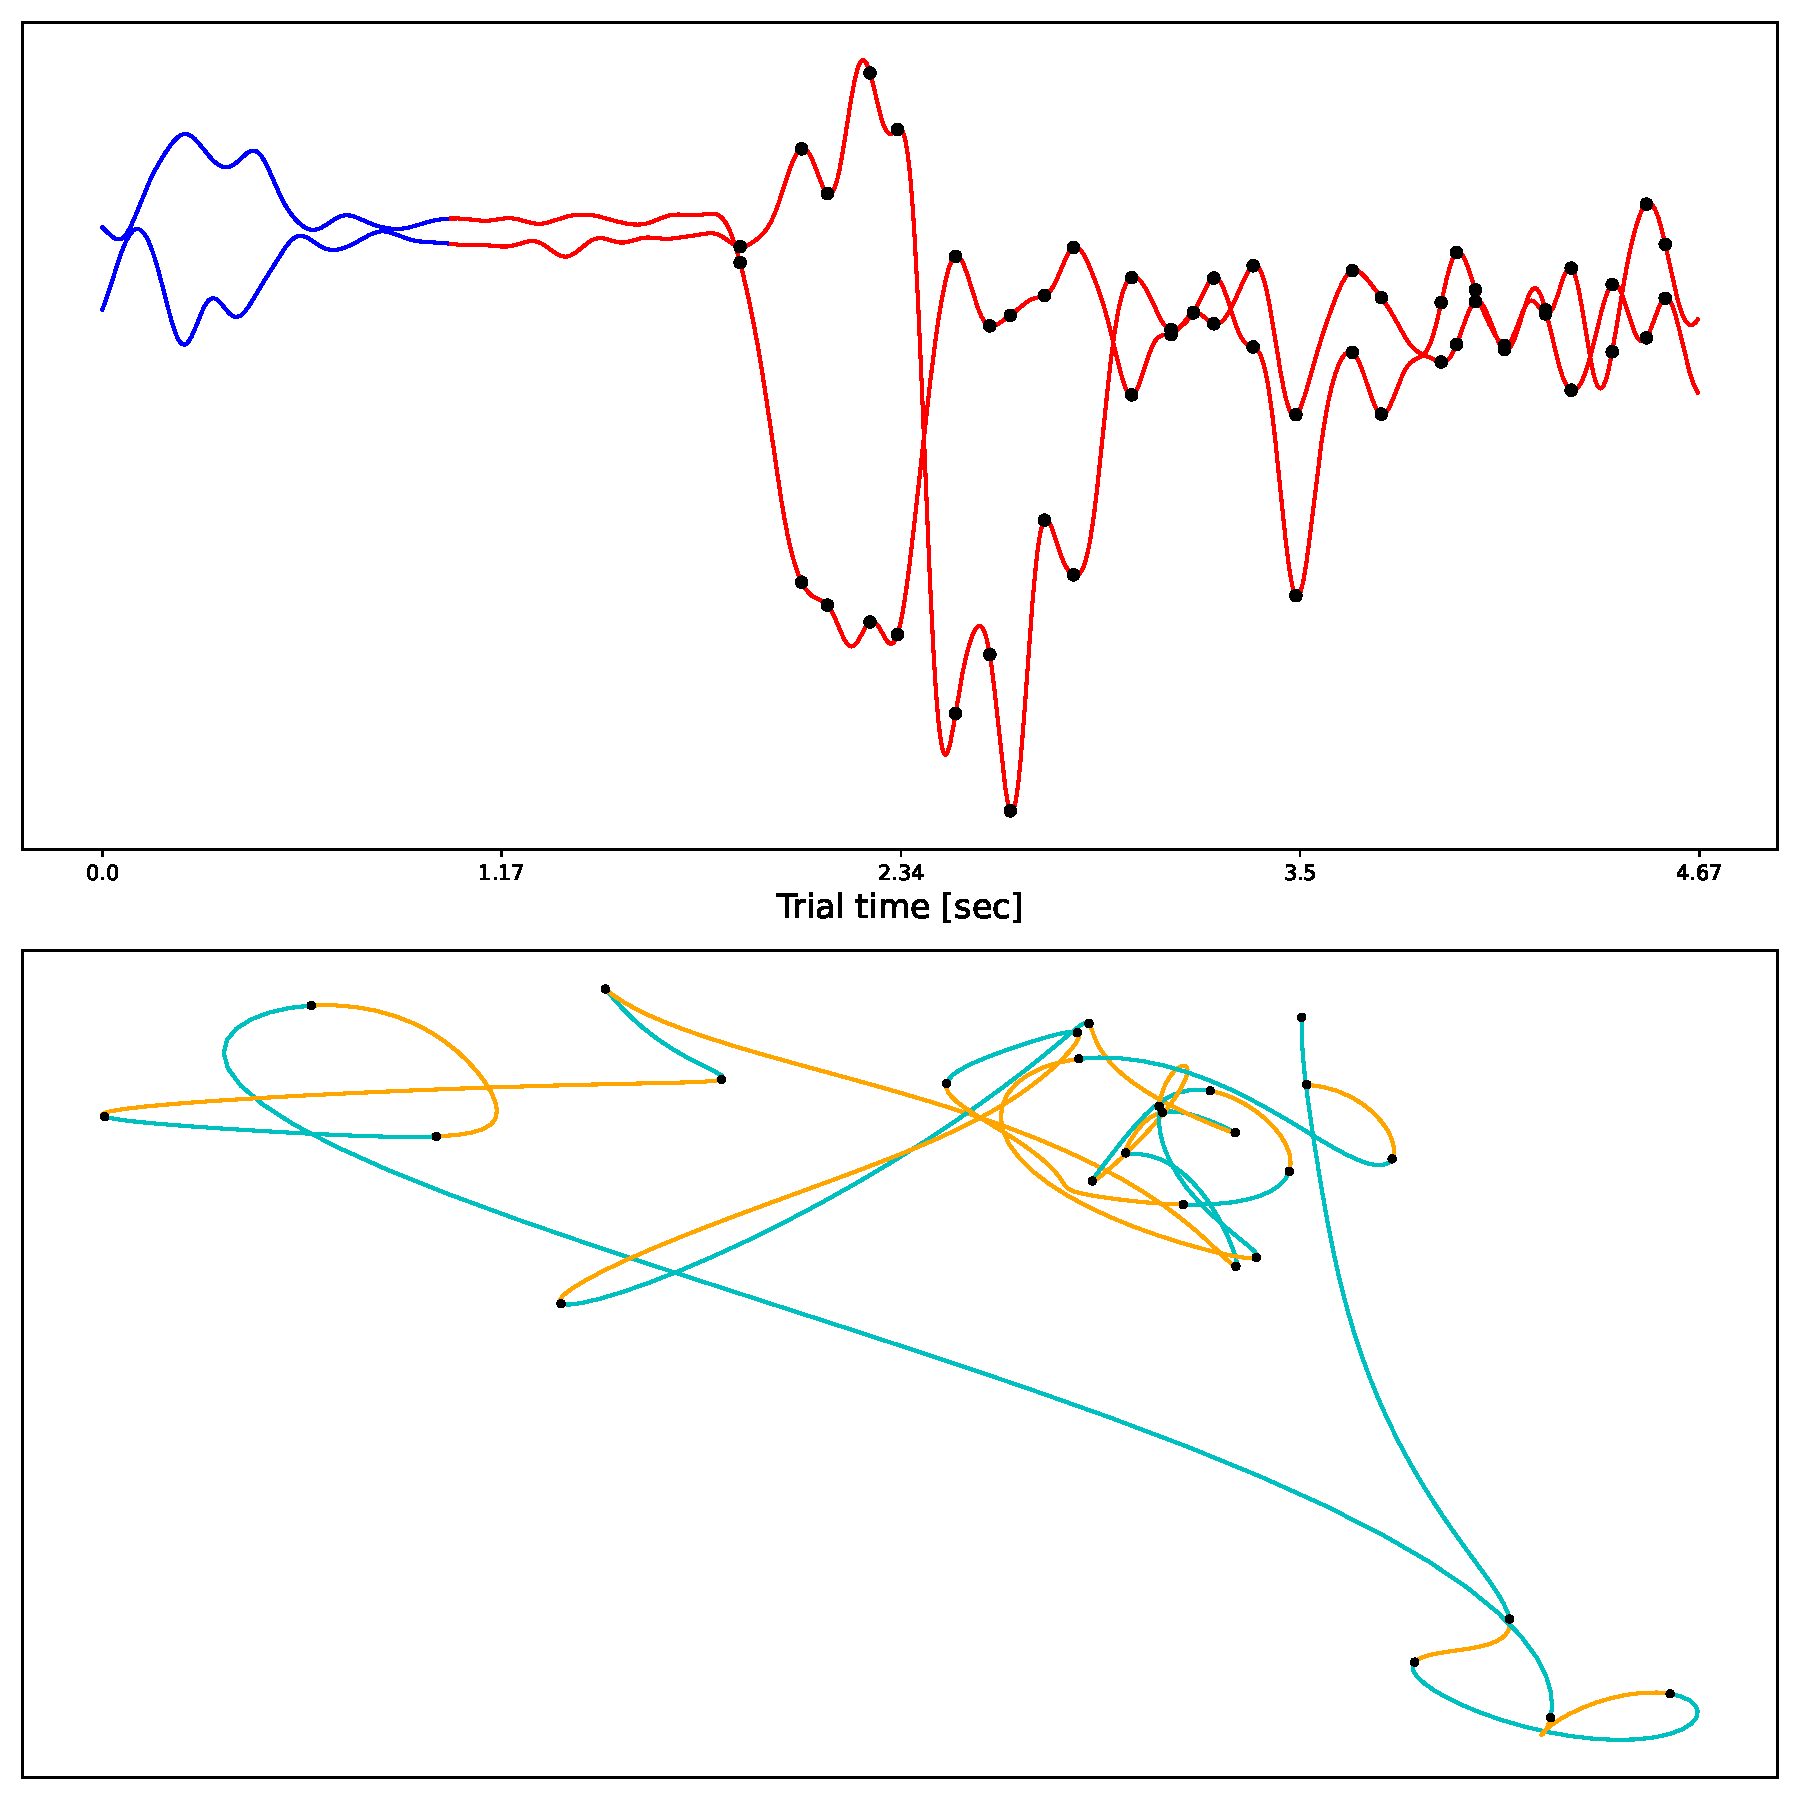
\includegraphics[width=0.7\textwidth]{basic_results/performance_over_blocks/example_path_segments.pdf}
    \caption[Example of a path segmented trial]{An example of path segmentation for one trajectory. Axes are removed to focus the example on the segmentation result. Top: The trajectory shown in red as an $x$ and $y$ coordinate over time. Path segments are defined as zero crossings of the trajectory's derivative. The black points identify zero crossings of the derivative, or maxima and minima in the trajectory. Bottom: The trajectory in the task space. We combine crossings which are near each other in time (below a set ``radius''), and exclude crossings below the 10th percentile of the max velocity in order to remove overly short segments. Resulting segments are shown in alternative blue and orange, with the black points highlighting segment switch points.}\label{fig:example_segments}
\end{figure}

\begin{figure}[!htb]%[H]
    \centering
    \includegraphics[width=1.0\textwidth]{basic_results/performance_over_blocks/path_segments_over_blocks.pdf}
    \caption[Trajectory segments over blocks]{Trajectory segments in task space, computed as described in the main text, averaged over each subjects' block of 12 trials, one trial per target in randomized order. Subjects with the most, least, and median numbers of hits are shown in green, orange, and blue, respectively. Log-fits are shown in matching colors for each of these subjects are shown to guide the eye. The mean over subjects per block is shown in dotted black.}\label{fig:path_segments_over_blocks}
\end{figure}

% We could look into the ``freezing degrees of freedom'' idea, defined as the size of the ``active'' EMG subspace within each trial. This could be done using NMF or PCA on each trial, e.g. many PCA components are active at once (how sparse are the component weights?), and how does this change over time? Sparsity (measured by the 1-norm) might imply that only a certain mode is active at a time, and this might change to more mixing over time. We would expect mixing to increase as people become more proficient and blend their activity modes together. This would be quite a rabbit hole, but interesting! We really want to know if people have distinct modes of activity early on, and how these blend into solutions over time. This is tricky to do, and currently lacking between the setup in the background chapters and the current results.

% \begin{figure}[!htb]%[H]
%     \centering
%     \includegraphics[width=1.0\textwidth]{basic_results/performance_over_blocks/reward_v_learning_rate.pdf}
%     \caption[Learning rates of path metrics versus reward]{Learning rates of path metrics versus reward}\label{fig:reward_v_learning_rate}
% \end{figure}

\begin{figure}[!htb]%[H]
    \centering
    \includegraphics[width=1.0\textwidth]{basic_results/performance_over_blocks/reward_v_metrics.pdf}
    \caption[Percent difference of path metrics versus reward]{For each task space metric (reach time, path length, and path segments), we take the percent difference of the means of the first 15 blocks and the last 15 blocks of trials for each subject, and plot these against each subjects reward.}\label{fig:reward_v_metrics}
\end{figure}

% \begin{able}%[H]
%     \begin{center}
%         \caption[Statistics of performance regression]{Statistics of performance regression}\label{tab:performance_stats}
%         \begin{tabular}{l | c}
%             \hline
%             $p$(Hit Learning Rate, Reward) & 0.177 \\
%             $p$(Reach time Learning Rate, Reward) & 0.215 \\
%             $p$(Path length Learning Rate, Reward) & 0.786 \\
%             $p$(Segment Learning Rate, Reward) & 0.072 \\
%             Adjusted R-squared & 0.058 \\
%             Prob (F-statistic) & 0.170
%         \end{tabular}
%     \end{center}
%   \end{table}
  
% mean_reward vs [hit_learning_rates, reach_time_learning_rates, path_length_learning_rates, segment_learning_rates]

% OLS Regression Results                            
% ==============================================================================
% Dep. Variable:                      y   R-squared:                       0.142
% Model:                            OLS   Adj. R-squared:                  0.058
% Method:                 Least Squares   F-statistic:                     1.693
% Date:                Wed, 14 Feb 2024   Prob (F-statistic):              0.170
% Time:                        10:31:57   Log-Likelihood:               -0.99915
% No. Observations:                  46   AIC:                             12.00
% Df Residuals:                      41   BIC:                             21.04
% Df Model:                           4                                         
% Covariance Type:            nonrobust                                         
% ==============================================================================
%                  coef    std err          t      P>|t|      [0.025      0.975]
% ------------------------------------------------------------------------------
% const          0.9233      0.114      8.083      0.000       0.693       1.054
% x1             0.0780      0.057      1.375      0.177      -0.037       0.193
% x2             0.7350      0.584      1.259      0.215      -0.444       1.914
% x3             0.0102      0.037      0.274      0.786      -0.065       0.085
% x4            -0.1088      0.059     -1.845      0.072      -0.228       0.010
% ==============================================================================
% Omnibus:                        4.990   Durbin-Watson:                   2.155
% Prob(Omnibus):                  0.083   Jarque-Bera (JB):                4.054
% Skew:                           0.477   Prob(JB):                        0.132
% Kurtosis:                       4.098   Cond. No.                         51.4
% ==============================================================================

% The learning rate for hits based on the logarithm fit to hit counts over blocks does not linearly correlate significantly with mean reward, indicating that the magnitude of the rate with which a subject accumulates hits over blocks does not necessarily lead to lower reward. This might be explained by the fact that some subjects start at high hit rate, meaning less learning is available to these subjects, meaning their learning rate is low despite their performance being high (reward being low). Note here that it may serve us well to look closely at subjects with high learning rates and high increases in performance over trials, as these subjects displayed the most learning, the largest spread in performance.

% \begin{figure}[!htb]%[H]
%     \centering
%     \includegraphics[width=1.0\textwidth]{basic_results/performance_over_blocks/velocity_v_reward.pdf}
%     \caption[Reach velocity versus reward]{Reach velocity versus reward. We could have used an exponential fit here, but linear without teh max and min subjects illustrates the idea well enough that higher performers on average move slower. This may seem counterintuitive but this is an aspect of a subject's ability to control their muscle activations. Lower peforming subjects tend to move more erratically, making more errors, while higher performers move less and thus on average move more slowly. We might initially question whether this is an artefact of the task, that subject variance induced by the EMG signal means subjects are noisier. But the left plot shows that we see no correlation between subjects' total variance in the calibration task and their performance. Also not that in the task, we standardize subject's EMG channels using their calibration variance, to reduce such effects (an unequal weighting of channels). We can also invoke Fitts' Law here? More accurate subjects move more slowly?}\label{fig:velocity}
% \end{figure}

% \begin{figure}[!htb]%[H]
%     \centering
%     \includegraphics[width=1.0\textwidth]{basic_results/performance_over_blocks/mean_rewards_vs_learning_rate.pdf}
%     \caption[Reward versus learning rate]{No correlation between the rate of hit accumulation and total reward.}\label{fig:mean_rewards_vs_learning_rate}
% \end{figure}


\section{Performance and Subject Attributes}

To assess whether any traits of our subjects and their experimental context correlated with their performance in the task, we asked subjects to complete a pre-experiment questionnaire, and we recorded experimental conditions. The following continuous attributes were recorded:

\begin{itemize}
    \item Time of day the data collection began. % no correlation
    \item Day order of the subject out of the cohort of 46 subjects. % no correlation
    \item Arm size: the circumference of a subject's dominant arm measured at a distance 10\% of their arm length (taken to be the distance between the elbow (olecranon) to the ulnar styloid) below the olecranon. % weak correlation!
    \item Hours of sleep reported the night before the experiment. % no correlation
\end{itemize}

We found no statistical significance in correlations with reward over subjects for any of these attributes except for arm size ($p=\num{3.17e-3}$), as shown in \Cref{fig:hour_of_day_vs_reward,fig:days_vs_reward,fig:arm_vs_reward,fig:sleep_vs_reward}. The following categorical attributes were collected:

\begin{itemize}
    \item Sex, male or female (options included non-binary, no subject chose these options). % significant difference in mean! This, we suspect, is explained by arm size
    \item Handedness, left or right. % none, though few left handed subjects
    \item Caffeine consumption day of the experiment; responses were grouped into ``high'' and ``low'' caffeine groups. %--- none 
    \item Sportsperson: ``regularly engaged in an activity that requires physicality and hand-eye coordination.'' % --- none 
    \item Dexterous: ``regularly engaged in a task considered dexterous.'' %--- none
\end{itemize}

The results of the categorical comparisons are shown in \Cref{fig:compare_subject_groups}. All categories show no significant difference in difference (by T-test) except for sex of the subjects. One explanation we can offer to explain this result is the difference in arm sizes for subjects who identified as female and male in the task. Those with arms of greater circumference appear to achieve higher reward in the task, and those with larger arms, on average, identified as male as shown in \Cref{fig:male_female_arms}. Those with larger arms achieving higher performance in the task may be explained by our flexible electrode array stretching to cover more of the arm. With more motor tissue (with more motor units) available for the task, subjects with larger arms may have an easier time decorrelating their EMG activity. We will explore this more deeply when we discuss our notion of ``subspace confinement'' in subsequent sections. For categories pertaining to non-anatomical attributes, we find no significant predictors of performance, which implies that our task provides a novel training ground for subjects.

\begin{figure}[!htb]%[H]
    \centering
    \includegraphics[width=1.0\textwidth]{basic_results/form_response/arm_vs_reward.pdf}
    \caption[Arm versus reward]{The circumference of each subject's dominant arm used in the task, measured 5cm below the tip of the elbow. We find a correlation (0.27, $p=\num{3.17e-3}$) in reward and arm size, as discussed in the main text.}\label{fig:arm_vs_reward}
\end{figure}

\begin{figure}[!htb]%[H]
    \centering
    \includegraphics[width=1.0\textwidth]{basic_results/form_response/days_vs_reward.pdf}
    \caption[Experiment day versus reward]{The date of each subject's experiment to highlight any trends in performance in the experiment over time. We find no significant correlation.}\label{fig:days_vs_reward}
\end{figure}

\begin{figure}[!htb]%[H]
    \centering
    \includegraphics[width=1.0\textwidth]{basic_results/form_response/hour_of_day_vs_reward.pdf}
    \caption[Hour of day versus reward]{The hour of day of each experiment to highlight and trends in performance with the time of day. We find no significant correlation.}\label{fig:hour_of_day_vs_reward}
\end{figure}

\begin{figure}[!htb]%[H]
    \centering
    \includegraphics[width=1.0\textwidth]{basic_results/form_response/sleep_vs_reward.pdf}
    \caption[Hours of sleep vs reward]{Self-reported hours of sleep the night before the experiment to highlight any trends in performance with sleep. We find no significant correlation.}\label{fig:sleep_vs_reward}
\end{figure}

\begin{figure}[!htb]%[H]
    \centering
    \includegraphics[width=1.0\textwidth]{basic_results/form_response/compare_subject_groups.pdf}
    \caption[Subject group comparisons]{Subject categories, self-reported, comparing means of each categorical pair. Differences in means are compared using a t-test. ``***'' indicates $p<\num{1e-3}$. We find significance only in the difference between male and female categories ($p=\num{2.84e-4}$) as discussed in the main text.}\label{fig:compare_subject_groups}
\end{figure}

\begin{figure}[!htb]%[H]
    \centering
    \includegraphics[width=0.6\textwidth]{basic_results/form_response/male_female_arms.pdf}
    \caption[Arm circumference and self-reported sex]{Plotting arm circumference between ``male'' and ``female'' groups to explain the correlation in performance with arm size with performance and sex with performance. We find a statistically significant difference in means of arm circumference between male and female groups ($p=\num{2.91e-6}$). The hypothetical advantage (in terms of EMG manifold) of larger arms is discussed in the main text.}\label{fig:male_female_arms}
\end{figure}


\section{Performance over Targets}

So far we have looked at mean rewards over all targets and subjects; we will now break results down across targets to assess any biases. As shown in \Cref{fig:hits_over_targets}, we find a statistically significant difference in the mean number of hits between the directly rightward target, Target 1, and the leftward targets 6, 7, 8, and 9. There is not an immediately obvious reason for this bias; this result might imply that with our method it is more likely that subjects' common movements, after decoding, lie in a leftward direction than a rightward one. That is, it is more likely for subjects to move leftward in the task space given their decoder, while it is least likely for subjects to move directly rightward. This hints at a major theme of this work: while we strongly support the continued development of a research program around electromyography to understand the computations underlying human learning, developing a finer-grained model of individual subjects' space of EMG activations is crucial to developing tasks with inter-subject comparability. This result in no way nullifies our findings here, but provides a context for them. Going forward, future experimentalists should work to develop a clear picture of subjects' EMG manifolds. This is a kind of bootstrapping problem; without running the task in the manner that we did, we would not have found such a bias (assuming it holds in all possible version of this experiment). In future iterations, it may prove fruitful to simulate task-space EMG projections to create decoders which explicitly balance activity between task states. Note, however, that subjects' natural biases within their EMG manifolds should not necessarily be completely removed, but appropriately leveraged for the goals of the experimental work.

% This should probably be log-transformed...?

\begin{figure}[!htb]%[H]
    \centering
    \begin{minipage}{1.0\textwidth}
        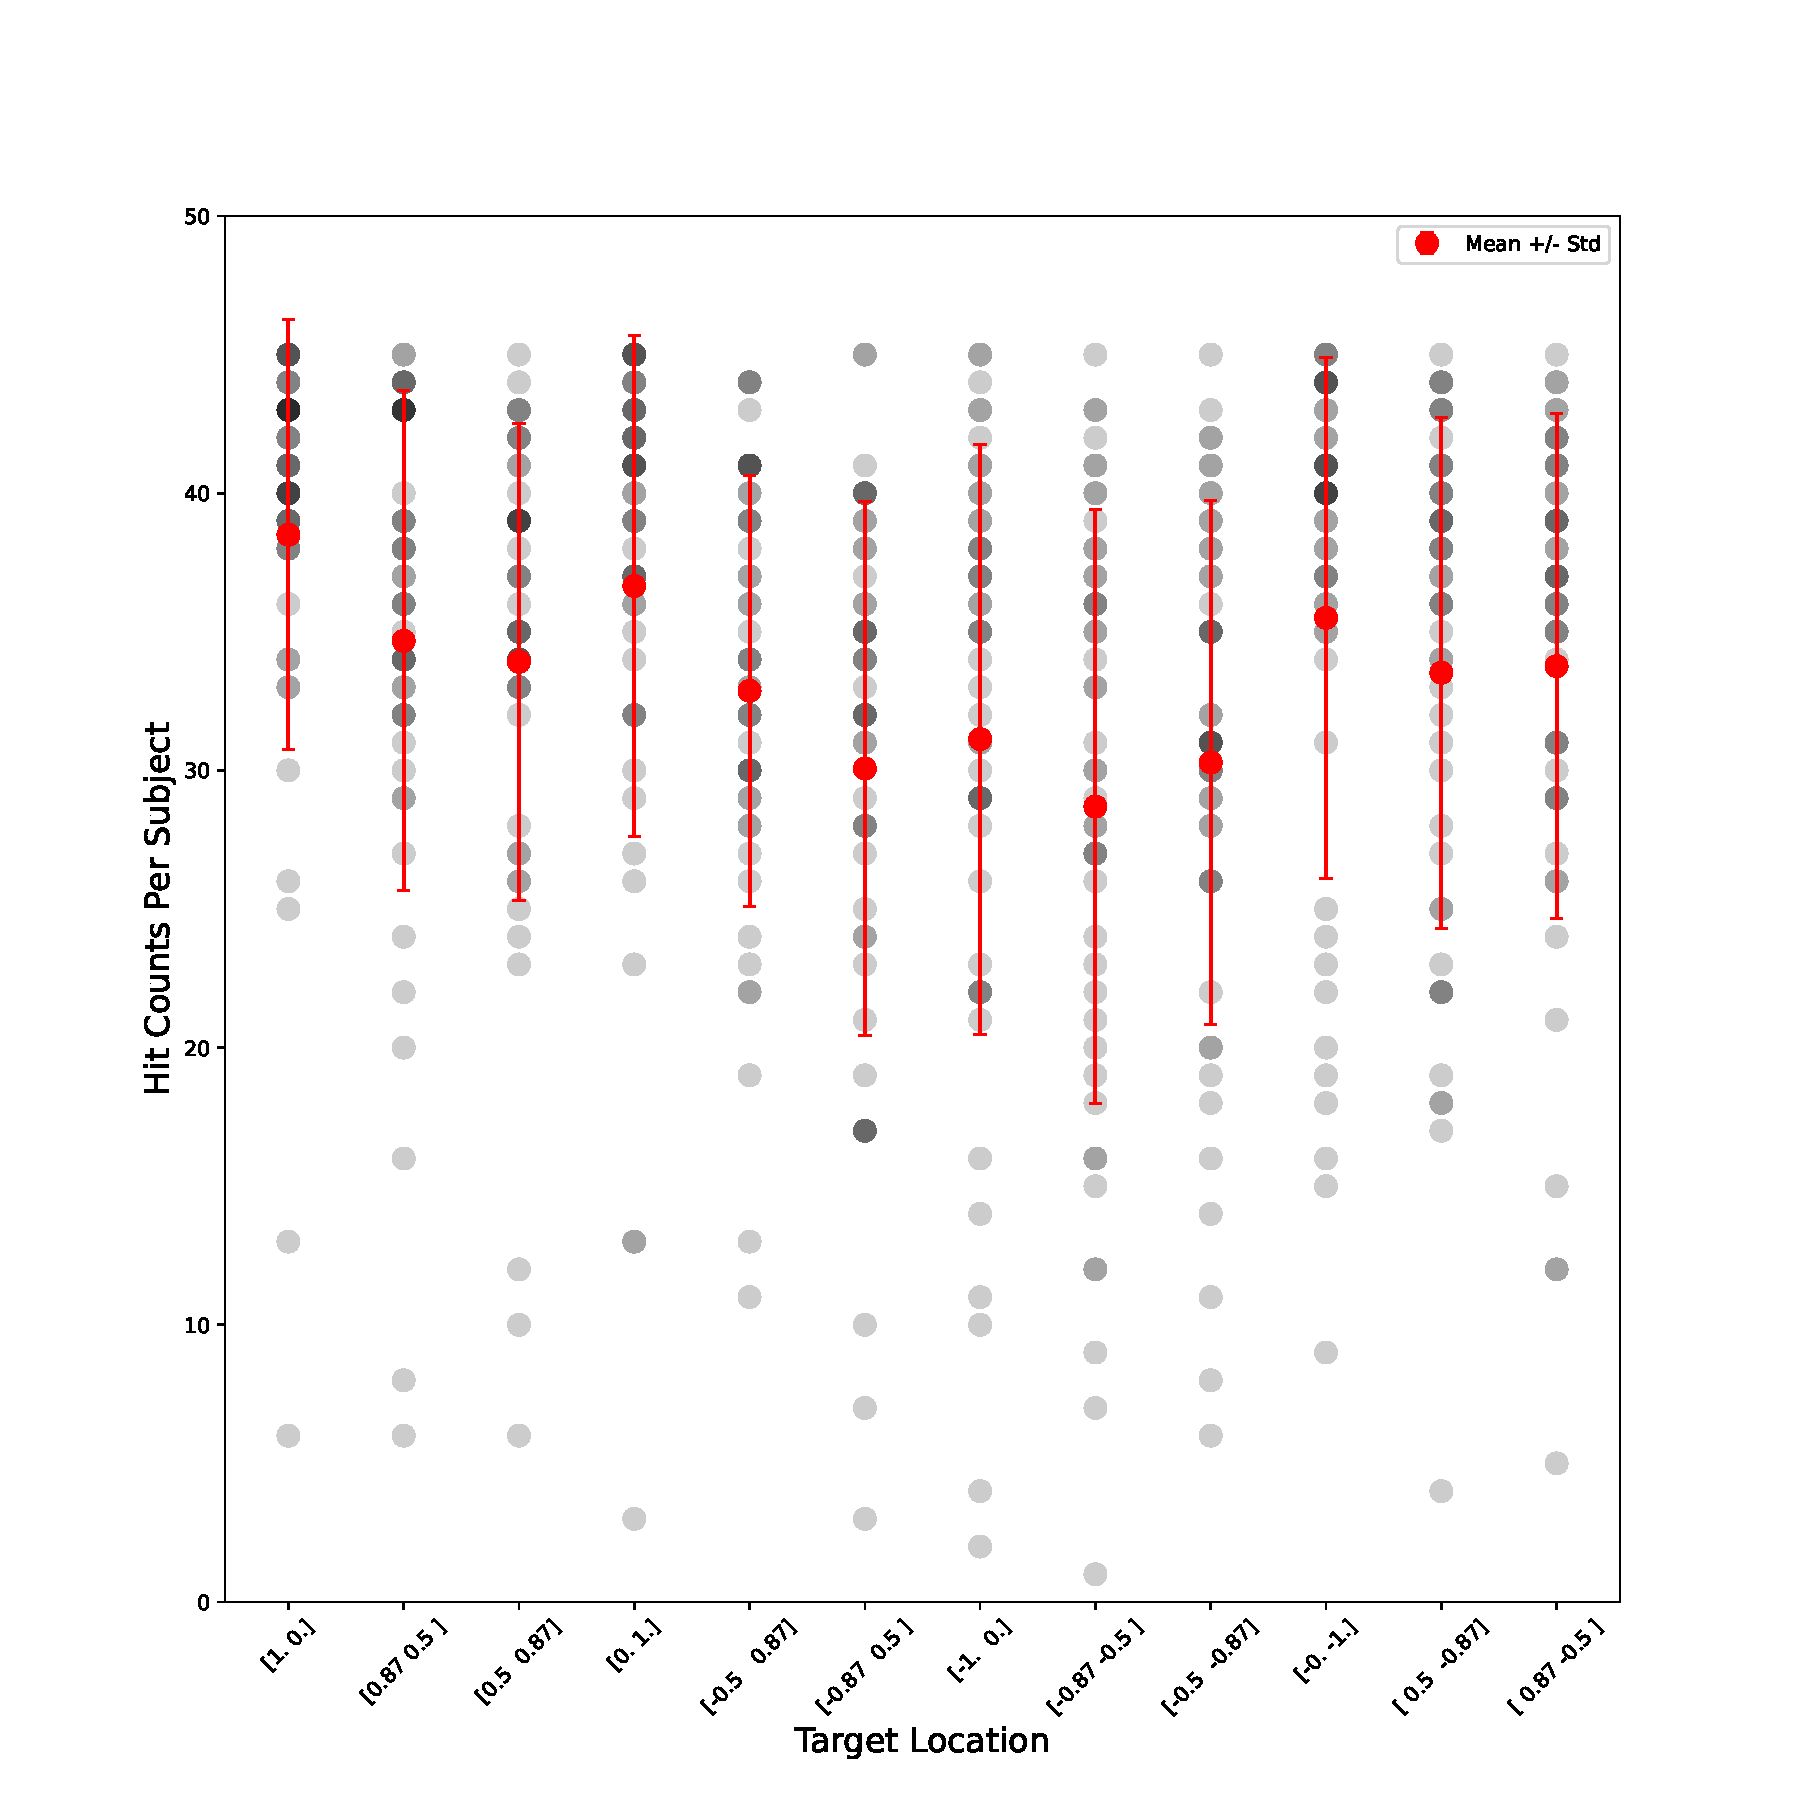
\includegraphics[width=1.0\textwidth]{basic_results/decoder_vs_performance/hits_over_targets.pdf}
        \subcaption{}
    \end{minipage}\\%
    \begin{minipage}{0.49\textwidth}
        \includegraphics[width=1.0\textwidth]{basic_results/decoder_vs_performance/target_means.pdf}
      \subcaption{}
    \end{minipage}
    \begin{minipage}{0.49\textwidth}
        \includegraphics[width=1.0\textwidth]{basic_results/decoder_vs_performance/target_hit_pvalues.pdf}
      \subcaption{}
    \end{minipage}
    \caption[Hits over Targets across subjects]{(a) Mean hit trial fractions for each subject, per target. Means over subjects are shown in red, with standard deviation error bars. (b) Mean hit trial fractions over subjects per target shown as the radius of each target marker to demonstrate in the task space where hits were more likely to occur across subjects. (c) Pairwise significance matrix reporting $p$-values from Tukey's honest significance test for multiple comparisons of hit trial fractions over individual targets to assess bias in target directions across subjects. We find that Target 1 (right) and Target 4 (up) are statistically significantly different from leftward targets.}\label{fig:hits_over_targets}
\end{figure}

One hypothesis is that our decoder generation method results in decoding which biases subjects' movements in particular directions. If these directions are advantageous to subject performance, some subjects may have an advantage based on their decoder in achieving more hits in the task. To investigate this, we can visualize subjects' decoders to look for a systematic bias in a particular direction, as shown in \Cref{fig:decoder_normality}. In the top left figure, we superimpose all subjects' decoders into two dimensions. That is, each arrow illustrates the direction in the task space which each electrode is mapped to. Qualitatively, we do not see any overt systematic bias across all subjects. This suggests, as previously discussed, that subjects' natural EMG manifolds are more likely to underlie task performance than their decoder. To test this hypothesis, we can ask how the action of the decoder shifts a uniform distribution of EMG signal in a unit cube ($[0,1]$) in $\mathcal{R}^{64}$. If we simulate EMG activity in the possible space of activation, sampling uniformly, and pass those activations through each subject's decoder we find, shown in \Cref{fig:decoder_normality}, that the result is a normal distribution (based on D'Agostino and Pearson's normality test) with significance for all subjects but one. Thus, our decoders effectively act as a spatial Gaussian blurring filter of our EMG signals in the task space. Subjects do not appear to be advantaged or disadvantaged by their decoders, only by their underlying EMG manifolds, which we will explore in depth in later sections.

\begin{figure}[!htb]%[H]
    \centering
    \includegraphics[width=1.0\textwidth]{basic_results/decoder_vs_performance/decoder_normality_test.pdf}
    \caption[Decoder normality test]{Top left: Superimposing all subject decoders into the task space, such that each arrow is the action of each electrode into the task space. Red markers are task target locations. Top right: Testing the effect of the decoder on uniformly sampled data from a unit cube $[0,1] \in \mathcal{R}^{64}$. Black markers are transformed samples from the EMG space into the task space from an example subject. Red markers are target locations in the task space. Bottom left: $p$ values from D'Agostino and Pearson's normality test for transformed uniform samples in $x$ and $y$. Red limits are 95\% significance. Bottom right: visualization of subjects with highest and lowest statistical significance, along with density plots of Gaussians with equivalent mean and variance to subject data to highlight how stringency of the normality test.}\label{fig:decoder_normality}
\end{figure}

Next, we ask whether the similarity of the $x$ and $y$ directions of each decoder correlates with performance in the task. If the decoder axes, which are non-orthogonal by design as discussed in \Cref{chap:methods}, are closely aligned in EMG space, this may disadvantage subjects beyond the ``blurring'' action of that decoder. As shown in \Cref{fig:decoder_cosine_vs_reward}, we found no significant correlation in the alignment, measure by cosine similarity, of the two decoder axes, and mean reward. A cosine similarity of 0 indicates that the decoder axes are perfectly orthogonal, while +1 and -1 indicates that these axes are perfectly parallel, in the same and opposite directions, respectively. 

% TODO: Plot the mean of all subjects decoder arrows, which may help to explain the bias towards the left hand side of the screen? However, this is a weird average to take since the order of EMG channels will differ. I would need to do this using some kind of density plot, overlaying each subject's decoder arrows in 2D. Probably more trouble than it's worth.

% Hypothesis: yes, decoder directions which happen to be oriented towards targets will make the learning problem easier, and thus correlate positively with performance. If the decoder directions are more/less aligned to the target directions, do subjects explore less/more? Is exploration (e.g. EMG variance) higher in subjects with misaligned decoders? Hypothesis: exploration will be lower in subjects with target-aligned decoders. Subjects make fewer incorrect movements, and thus are induced to explore less.

% \begin{figure}[!htb]%[H]
%     \centering
%     \includegraphics[width=0.7\textwidth]{basic_results/decoder_vs_performance/decoder_arrows.pdf}
%     \caption[Example decoder directions in 2D.]{Example decoders directions in 2D.}\label{fig:decoder_arrows}
% \end{figure}

\begin{figure}[!htb]%[H]
    \centering
    \includegraphics[width=1.0\textwidth]{basic_results/decoder_vs_performance/decoder_cosine_vs_reward.pdf}
    \caption[Decoder cosine similarity versus reward]{Cosine similarity between the $x$ and $y$ EMG-to-force decoder axes in EMG space. A cosine similarity of +1/-1 indicates that the two vectors are parallel/antiparallel, producing equal/opposite task actions for the same EMG activity ($T_x = T_y$ or $T_x = -T_y$). A cosine similarity of 0 indicates that the decoder directions are orthogonal, producing task action in $x$ direction with a certain EMG activity produces no activity in the $y$ direction or vice versa. The $x$ and $y$ actions are decoupled. We ask whether cosine similarity is predictive of task success, in terms of the numbers of mean task reward. We find no significant correlation, implying that decoder cosine similarity is not predictive of task success.}\label{fig:decoder_cosine_vs_reward}
\end{figure}

% \begin{figure}[!htb]%[H]
%     \centering
%     \includegraphics[width=0.8\textwidth]{basic_results/decoder_vs_performance/mean_decoder.pdf}
%     \caption[Decoder normality testing]{Average decoder over subjects}\label{fig:mean_decoder}
% \end{figure}


\section{Task Variance over Trials}

As discussed in reference to \Cref{sec:performance_over_blocks}, we have seen that performance appears to be underpinned to some extent by lowering general variability in the task space. How this task variability relates to variability of subjects' EMG will be explored deeply in later chapters. Looking at the example task trajectories for three subjects (maximum, minimum, and median reward) in \Cref{fig:mean_trajectories}, mean trajectories are shown in color and have been interpolated in time. Higher performing subjects tend to have less erratic movements, and seem to use the dominant directions of their underlying EMG manifold, projected onto the task plane, to their advantage. This can be seen for example in the three dominant directions in the maximum reward subject. These example trajectories, particularly the target means, give a warped (in time) perspective of the task space variability as more variability timepoints will have an outweighed effect on the mean when interpolated.

To compare trajectories over time and assess variability across learning, we rotate trajectories towards a single target, Target 1 directly to the right, to compare like-for-like. An example of this action of rotation is shown in \Cref{fig:rotated_trajectories}. In \Cref{fig:example_trajectories}, we show the $y$ coordinate of rotated trajectories for each target over 5 ``chunks'' of 9 blocks (108 trials) each. The $y$ coordinate is used here as the $x$ coordinate, post-rotation, is meant to increase from 0 to 1 in order to reach the target. The $y$ coordinate, under rotation, should remain at 0 to reach Target 1. This gives us a straightforward signal of movement variability over trials. This is clear in the example of \Cref{fig:trajectory_variance}, where qualitatively we see that the $y$ coordinate variability decreasing over time.

To compare across subjects, in \Cref{fig:trajectory_variance} we plot the median variance and it's inter-quartile range over subjects of the rotated $y$ coordinate. Qualitatively we see that variance over subjects decreases across learning, as subjects discover and ``hone'' their task solutions. Quantitatively, we run a multiple comparison Tukey test to compare mean variances over subjects and targets across trial block groups. We find significant evidence that means of the first and last group of trial blocks are not identical, supporting the fact that task variance decreases across learning over all subjects. This summarizes a general result from task learning, that subjects learn to generate less variable movements across practice. The question remaining is not \textit{if} subjects lower the variance of their movements across learning, but \textit{how} subjects achieve this reduction in variance by changing their patterns of muscle activations. In the next sections we will explore the structure of subject EMG variability in more detail.


\begin{figure}[!htb]%[H]
    \centering
    \includegraphics[width=\textwidth]{basic_results/mean_trajectories/mean_trajectories.pdf}
    \caption[Example task trajectories and means per target]{Example task trajectories for three subjects: maximum, minimum, and median reward. Trajectories are shown in black, while for each target we interpolate trajectories in time to time-normalize them in order to take means of per-target trajectories. This gives a coarse impression of mean trajectories, though the interpolation scheme will overweight the effect of high variability movements, as seen in the minimum reward subject (bottom).}\label{fig:mean_trajectories}
\end{figure}


\begin{figure}[!htb]%[H]
    \centering
    \includegraphics[width=\textwidth]{basic_results/trajectory_variance/rotated_trajectories.pdf}
    \caption[Example rotated trajectories, single block]{An example of a single subject and block of trial's targets in task space. Left: Original task space trajectories. Right: Rotated trajectories to compare all trials to Target 1. Targets shown in red.}\label{fig:rotated_trajectories}
\end{figure}


\begin{sidewaysfigure}[!htb]
    \centering
    \includegraphics[width=\textwidth]{basic_results/trajectory_variance/subject_example_trajectory_variance.pdf}
    \caption[Example rotated trajectories, all blocks]{Example rotated trajectories for a single subject over five groups of trial blocks (108 trials per group) broken down by target for the $y$ coordinate. The histograms collect samples over time to highlight the decrease in variance over trials.}\label{fig:example_trajectories}
\end{sidewaysfigure}


\begin{figure}[!htb]%[H]
    \centering
    \begin{minipage}{1.0\textwidth}
    \includegraphics[width=1.0\textwidth]{basic_results/trajectory_variance/trajectory_variance_blocks.pdf}\subcaption{}
    \end{minipage}\\%
    \begin{minipage}{0.7\textwidth}
        \includegraphics[width=1.0\textwidth]{basic_results/trajectory_variance/trajectory_variance_pvalues.png}
      \subcaption{}
    \end{minipage}
    \caption[Median and IQR of trajectory variance over blocks and subjects]{(a) Trajectory variance over block groups (108 trials each) with medians and IQR over subjects. We see variance in the task space decreasing over learning. (b) Multiple comparison Tukey test for the mean variance over subjects across learning, comparing trial groups pairwise. We find significance in rejection of the null hypothesis that the mean of variance of the first and last trial groups is identical.}\label{fig:trajectory_variance}
\end{figure}


% \begin{figure}[!htb]%[H]
%     \centering
%     \includegraphics[width=1.0\textwidth]{basic_results/trajectory_variance/trajectory_variance_blocks.pdf}
%     \caption[Median and IQR of trajectory variance over blocks and subjects]{Trajectory variance over blocks, median, IQR over subjects}\label{fig:trajectory_variance}
% \end{figure}


% cut this as it's shit
% \begin{figure}[!htb]%[H]
%     \centering
%     \begin{minipage}{0.9\textwidth}
%         \includegraphics[width=\textwidth]{basic_results/trajectory_variance/trajectory_r_squared_fit.pdf}
%         \subcaption{}
%     \end{minipage}\\%
%     \begin{minipage}{0.9\textwidth}
%         \includegraphics[width=0.8\textwidth]{basic_results/trajectory_variance/trajectory_variance_slope.pdf}
%       \subcaption{}
%     \end{minipage}
%     \caption[Trajectory variance statistics]{Trajectory variance statistics}\label{fig:trajectory_variance_fits}
% \end{figure}


\cleardoublepage\printendnotes%
\ifSubfilesClassLoaded{%
    \newpage%
    \bibliography{../bib/bibliography}%
}{}%
\end{document}